% Caption: Anyon braiding in 2+1D. Left: a single exchange (half-braid) of two
% quasiparticles acquires a statistical phase $e^{i\pi/m}$. Right: a full
% monodromy (one particle encircles the other) yields $e^{2\pi i/m}$, the
% square of the exchange phase. Crossings are drawn with the knot convention
% (white gap = under-strand).
%
% Usage: % Caption: Anyon braiding in 2+1D. Left: a single exchange (half-braid) of two
% quasiparticles acquires a statistical phase $e^{i\pi/m}$. Right: a full
% monodromy (one particle encircles the other) yields $e^{2\pi i/m}$, the
% square of the exchange phase. Crossings are drawn with the knot convention
% (white gap = under-strand).
%
% Usage: % Caption: Anyon braiding in 2+1D. Left: a single exchange (half-braid) of two
% quasiparticles acquires a statistical phase $e^{i\pi/m}$. Right: a full
% monodromy (one particle encircles the other) yields $e^{2\pi i/m}$, the
% square of the exchange phase. Crossings are drawn with the knot convention
% (white gap = under-strand).
%
% Usage: % Caption: Anyon braiding in 2+1D. Left: a single exchange (half-braid) of two
% quasiparticles acquires a statistical phase $e^{i\pi/m}$. Right: a full
% monodromy (one particle encircles the other) yields $e^{2\pi i/m}$, the
% square of the exchange phase. Crossings are drawn with the knot convention
% (white gap = under-strand).
%
% Usage: \input{figures/f_anyon_braid.tex}
% Requires: \usepackage{tikz}

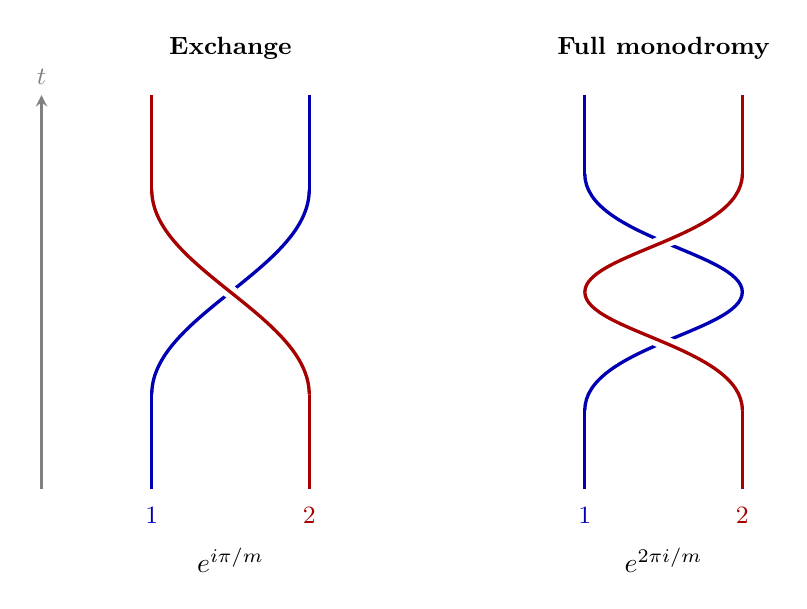
\begin{tikzpicture}[scale=1.0, thick,
    particle1/.style={very thick, blue!70!black},
    particle2/.style={very thick, red!65!black},
    gap/.style={white, line width=5pt}]

  %% ===== LEFT PANEL: EXCHANGE (half-braid) =====
  \begin{scope}[shift={(0,0)}]

    % Time axis
    \draw[-stealth, gray] (-0.6, 0) -- (-0.6, 5.0) node[above, font=\small] {$t$};

    % Particle 1: starts left, ends right
    \draw[particle1] (0.8, 0) -- (0.8, 1.2);
    \draw[particle1] (0.8, 1.2) .. controls (0.8, 2.2) and (2.8, 2.8) .. (2.8, 3.8);
    \draw[particle1] (2.8, 3.8) -- (2.8, 5.0);

    % Particle 2: starts right, ends left — with under-crossing
    \draw[particle2] (2.8, 0) -- (2.8, 1.2);
    % Draw gap (white) where particle 2 passes under particle 1
    \draw[gap] (2.8, 1.2) .. controls (2.8, 2.2) and (0.8, 2.8) .. (0.8, 3.8);
    % Redraw particle 2 after gap
    \draw[particle2] (2.8, 1.2) .. controls (2.8, 2.2) and (0.8, 2.8) .. (0.8, 3.8);
    \draw[particle2] (0.8, 3.8) -- (0.8, 5.0);

    % Particle labels
    \node[below, font=\small, blue!70!black] at (0.8, -0.1) {$1$};
    \node[below, font=\small, red!65!black] at (2.8, -0.1) {$2$};

    % Phase label
    \node[font=\normalsize] at (1.8, -0.9) {$e^{i\pi/m}$};

    % Panel title
    \node[font=\small\bfseries] at (1.8, 5.6) {Exchange};
  \end{scope}

  %% ===== RIGHT PANEL: FULL MONODROMY (double braid) =====
  \begin{scope}[shift={(5.5,0)}]

    % Particle 1: stays roughly in place (slight wobble for clarity)
    \draw[particle1] (0.8, 0) -- (0.8, 1.0);
    % First crossing: particle 1 goes right, particle 2 goes left
    \draw[particle1] (0.8, 1.0) .. controls (0.8, 1.8) and (2.8, 2.0) .. (2.8, 2.5);
    % Second crossing: particle 1 returns left
    \draw[particle1] (2.8, 2.5) .. controls (2.8, 3.0) and (0.8, 3.2) .. (0.8, 4.0);
    \draw[particle1] (0.8, 4.0) -- (0.8, 5.0);

    % Particle 2: complementary path with under-crossings
    \draw[particle2] (2.8, 0) -- (2.8, 1.0);

    % First under-crossing (particle 2 goes under particle 1)
    \draw[gap] (2.8, 1.0) .. controls (2.8, 1.8) and (0.8, 2.0) .. (0.8, 2.5);
    \draw[particle2] (2.8, 1.0) .. controls (2.8, 1.8) and (0.8, 2.0) .. (0.8, 2.5);

    % Second under-crossing (particle 2 goes under particle 1 again)
    \draw[gap] (0.8, 2.5) .. controls (0.8, 3.0) and (2.8, 3.2) .. (2.8, 4.0);
    \draw[particle2] (0.8, 2.5) .. controls (0.8, 3.0) and (2.8, 3.2) .. (2.8, 4.0);

    \draw[particle2] (2.8, 4.0) -- (2.8, 5.0);

    % Particle labels
    \node[below, font=\small, blue!70!black] at (0.8, -0.1) {$1$};
    \node[below, font=\small, red!65!black] at (2.8, -0.1) {$2$};

    % Phase label
    \node[font=\normalsize] at (1.8, -0.9) {$e^{2\pi i/m}$};

    % Panel title
    \node[font=\small\bfseries] at (1.8, 5.6) {Full monodromy};
  \end{scope}

\end{tikzpicture}

% Requires: \usepackage{tikz}

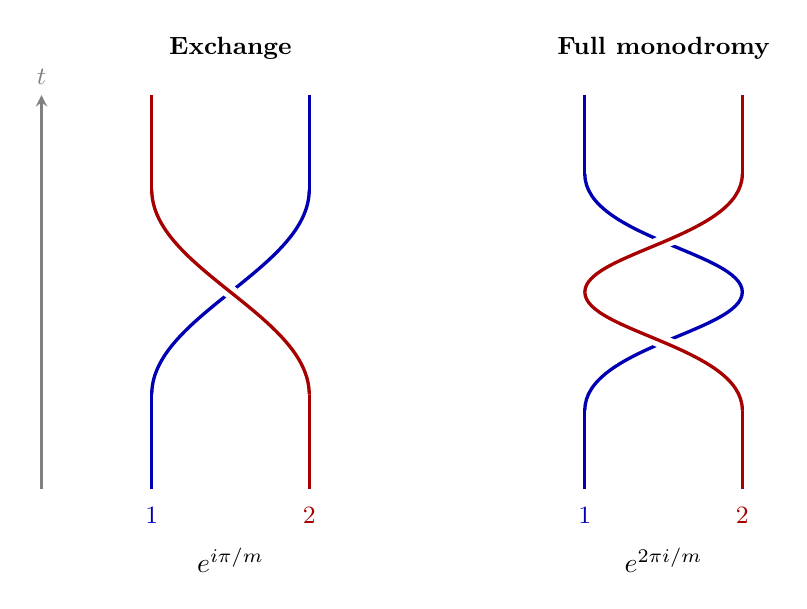
\begin{tikzpicture}[scale=1.0, thick,
    particle1/.style={very thick, blue!70!black},
    particle2/.style={very thick, red!65!black},
    gap/.style={white, line width=5pt}]

  %% ===== LEFT PANEL: EXCHANGE (half-braid) =====
  \begin{scope}[shift={(0,0)}]

    % Time axis
    \draw[-stealth, gray] (-0.6, 0) -- (-0.6, 5.0) node[above, font=\small] {$t$};

    % Particle 1: starts left, ends right
    \draw[particle1] (0.8, 0) -- (0.8, 1.2);
    \draw[particle1] (0.8, 1.2) .. controls (0.8, 2.2) and (2.8, 2.8) .. (2.8, 3.8);
    \draw[particle1] (2.8, 3.8) -- (2.8, 5.0);

    % Particle 2: starts right, ends left — with under-crossing
    \draw[particle2] (2.8, 0) -- (2.8, 1.2);
    % Draw gap (white) where particle 2 passes under particle 1
    \draw[gap] (2.8, 1.2) .. controls (2.8, 2.2) and (0.8, 2.8) .. (0.8, 3.8);
    % Redraw particle 2 after gap
    \draw[particle2] (2.8, 1.2) .. controls (2.8, 2.2) and (0.8, 2.8) .. (0.8, 3.8);
    \draw[particle2] (0.8, 3.8) -- (0.8, 5.0);

    % Particle labels
    \node[below, font=\small, blue!70!black] at (0.8, -0.1) {$1$};
    \node[below, font=\small, red!65!black] at (2.8, -0.1) {$2$};

    % Phase label
    \node[font=\normalsize] at (1.8, -0.9) {$e^{i\pi/m}$};

    % Panel title
    \node[font=\small\bfseries] at (1.8, 5.6) {Exchange};
  \end{scope}

  %% ===== RIGHT PANEL: FULL MONODROMY (double braid) =====
  \begin{scope}[shift={(5.5,0)}]

    % Particle 1: stays roughly in place (slight wobble for clarity)
    \draw[particle1] (0.8, 0) -- (0.8, 1.0);
    % First crossing: particle 1 goes right, particle 2 goes left
    \draw[particle1] (0.8, 1.0) .. controls (0.8, 1.8) and (2.8, 2.0) .. (2.8, 2.5);
    % Second crossing: particle 1 returns left
    \draw[particle1] (2.8, 2.5) .. controls (2.8, 3.0) and (0.8, 3.2) .. (0.8, 4.0);
    \draw[particle1] (0.8, 4.0) -- (0.8, 5.0);

    % Particle 2: complementary path with under-crossings
    \draw[particle2] (2.8, 0) -- (2.8, 1.0);

    % First under-crossing (particle 2 goes under particle 1)
    \draw[gap] (2.8, 1.0) .. controls (2.8, 1.8) and (0.8, 2.0) .. (0.8, 2.5);
    \draw[particle2] (2.8, 1.0) .. controls (2.8, 1.8) and (0.8, 2.0) .. (0.8, 2.5);

    % Second under-crossing (particle 2 goes under particle 1 again)
    \draw[gap] (0.8, 2.5) .. controls (0.8, 3.0) and (2.8, 3.2) .. (2.8, 4.0);
    \draw[particle2] (0.8, 2.5) .. controls (0.8, 3.0) and (2.8, 3.2) .. (2.8, 4.0);

    \draw[particle2] (2.8, 4.0) -- (2.8, 5.0);

    % Particle labels
    \node[below, font=\small, blue!70!black] at (0.8, -0.1) {$1$};
    \node[below, font=\small, red!65!black] at (2.8, -0.1) {$2$};

    % Phase label
    \node[font=\normalsize] at (1.8, -0.9) {$e^{2\pi i/m}$};

    % Panel title
    \node[font=\small\bfseries] at (1.8, 5.6) {Full monodromy};
  \end{scope}

\end{tikzpicture}

% Requires: \usepackage{tikz}

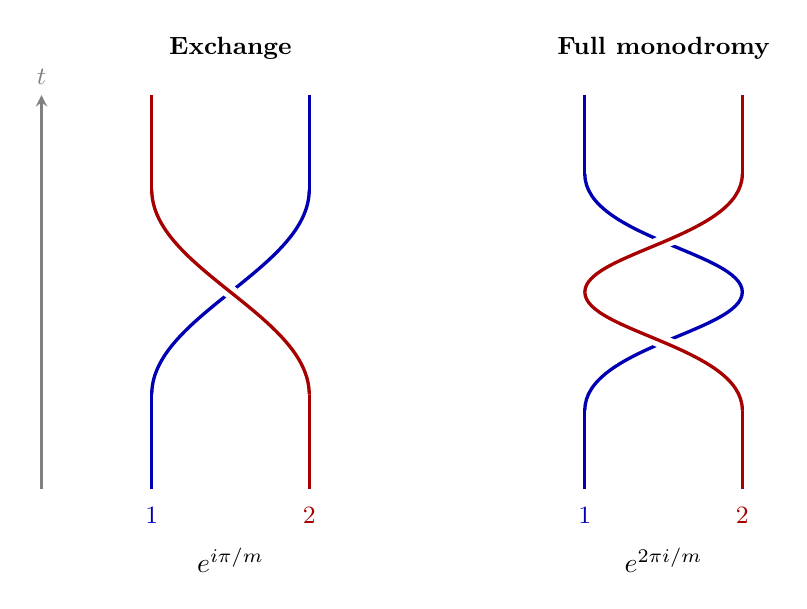
\begin{tikzpicture}[scale=1.0, thick,
    particle1/.style={very thick, blue!70!black},
    particle2/.style={very thick, red!65!black},
    gap/.style={white, line width=5pt}]

  %% ===== LEFT PANEL: EXCHANGE (half-braid) =====
  \begin{scope}[shift={(0,0)}]

    % Time axis
    \draw[-stealth, gray] (-0.6, 0) -- (-0.6, 5.0) node[above, font=\small] {$t$};

    % Particle 1: starts left, ends right
    \draw[particle1] (0.8, 0) -- (0.8, 1.2);
    \draw[particle1] (0.8, 1.2) .. controls (0.8, 2.2) and (2.8, 2.8) .. (2.8, 3.8);
    \draw[particle1] (2.8, 3.8) -- (2.8, 5.0);

    % Particle 2: starts right, ends left — with under-crossing
    \draw[particle2] (2.8, 0) -- (2.8, 1.2);
    % Draw gap (white) where particle 2 passes under particle 1
    \draw[gap] (2.8, 1.2) .. controls (2.8, 2.2) and (0.8, 2.8) .. (0.8, 3.8);
    % Redraw particle 2 after gap
    \draw[particle2] (2.8, 1.2) .. controls (2.8, 2.2) and (0.8, 2.8) .. (0.8, 3.8);
    \draw[particle2] (0.8, 3.8) -- (0.8, 5.0);

    % Particle labels
    \node[below, font=\small, blue!70!black] at (0.8, -0.1) {$1$};
    \node[below, font=\small, red!65!black] at (2.8, -0.1) {$2$};

    % Phase label
    \node[font=\normalsize] at (1.8, -0.9) {$e^{i\pi/m}$};

    % Panel title
    \node[font=\small\bfseries] at (1.8, 5.6) {Exchange};
  \end{scope}

  %% ===== RIGHT PANEL: FULL MONODROMY (double braid) =====
  \begin{scope}[shift={(5.5,0)}]

    % Particle 1: stays roughly in place (slight wobble for clarity)
    \draw[particle1] (0.8, 0) -- (0.8, 1.0);
    % First crossing: particle 1 goes right, particle 2 goes left
    \draw[particle1] (0.8, 1.0) .. controls (0.8, 1.8) and (2.8, 2.0) .. (2.8, 2.5);
    % Second crossing: particle 1 returns left
    \draw[particle1] (2.8, 2.5) .. controls (2.8, 3.0) and (0.8, 3.2) .. (0.8, 4.0);
    \draw[particle1] (0.8, 4.0) -- (0.8, 5.0);

    % Particle 2: complementary path with under-crossings
    \draw[particle2] (2.8, 0) -- (2.8, 1.0);

    % First under-crossing (particle 2 goes under particle 1)
    \draw[gap] (2.8, 1.0) .. controls (2.8, 1.8) and (0.8, 2.0) .. (0.8, 2.5);
    \draw[particle2] (2.8, 1.0) .. controls (2.8, 1.8) and (0.8, 2.0) .. (0.8, 2.5);

    % Second under-crossing (particle 2 goes under particle 1 again)
    \draw[gap] (0.8, 2.5) .. controls (0.8, 3.0) and (2.8, 3.2) .. (2.8, 4.0);
    \draw[particle2] (0.8, 2.5) .. controls (0.8, 3.0) and (2.8, 3.2) .. (2.8, 4.0);

    \draw[particle2] (2.8, 4.0) -- (2.8, 5.0);

    % Particle labels
    \node[below, font=\small, blue!70!black] at (0.8, -0.1) {$1$};
    \node[below, font=\small, red!65!black] at (2.8, -0.1) {$2$};

    % Phase label
    \node[font=\normalsize] at (1.8, -0.9) {$e^{2\pi i/m}$};

    % Panel title
    \node[font=\small\bfseries] at (1.8, 5.6) {Full monodromy};
  \end{scope}

\end{tikzpicture}

% Requires: \usepackage{tikz}

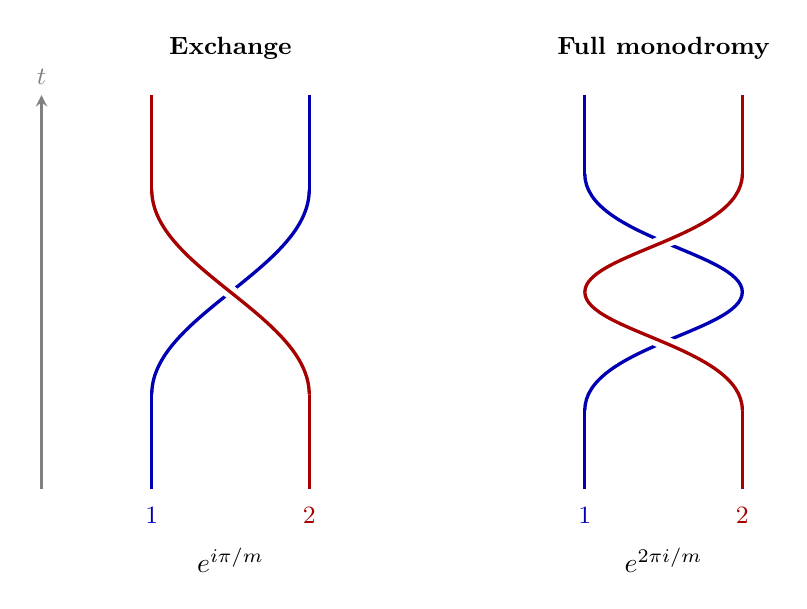
\begin{tikzpicture}[scale=1.0, thick,
    particle1/.style={very thick, blue!70!black},
    particle2/.style={very thick, red!65!black},
    gap/.style={white, line width=5pt}]

  %% ===== LEFT PANEL: EXCHANGE (half-braid) =====
  \begin{scope}[shift={(0,0)}]

    % Time axis
    \draw[-stealth, gray] (-0.6, 0) -- (-0.6, 5.0) node[above, font=\small] {$t$};

    % Particle 1: starts left, ends right
    \draw[particle1] (0.8, 0) -- (0.8, 1.2);
    \draw[particle1] (0.8, 1.2) .. controls (0.8, 2.2) and (2.8, 2.8) .. (2.8, 3.8);
    \draw[particle1] (2.8, 3.8) -- (2.8, 5.0);

    % Particle 2: starts right, ends left — with under-crossing
    \draw[particle2] (2.8, 0) -- (2.8, 1.2);
    % Draw gap (white) where particle 2 passes under particle 1
    \draw[gap] (2.8, 1.2) .. controls (2.8, 2.2) and (0.8, 2.8) .. (0.8, 3.8);
    % Redraw particle 2 after gap
    \draw[particle2] (2.8, 1.2) .. controls (2.8, 2.2) and (0.8, 2.8) .. (0.8, 3.8);
    \draw[particle2] (0.8, 3.8) -- (0.8, 5.0);

    % Particle labels
    \node[below, font=\small, blue!70!black] at (0.8, -0.1) {$1$};
    \node[below, font=\small, red!65!black] at (2.8, -0.1) {$2$};

    % Phase label
    \node[font=\normalsize] at (1.8, -0.9) {$e^{i\pi/m}$};

    % Panel title
    \node[font=\small\bfseries] at (1.8, 5.6) {Exchange};
  \end{scope}

  %% ===== RIGHT PANEL: FULL MONODROMY (double braid) =====
  \begin{scope}[shift={(5.5,0)}]

    % Particle 1: stays roughly in place (slight wobble for clarity)
    \draw[particle1] (0.8, 0) -- (0.8, 1.0);
    % First crossing: particle 1 goes right, particle 2 goes left
    \draw[particle1] (0.8, 1.0) .. controls (0.8, 1.8) and (2.8, 2.0) .. (2.8, 2.5);
    % Second crossing: particle 1 returns left
    \draw[particle1] (2.8, 2.5) .. controls (2.8, 3.0) and (0.8, 3.2) .. (0.8, 4.0);
    \draw[particle1] (0.8, 4.0) -- (0.8, 5.0);

    % Particle 2: complementary path with under-crossings
    \draw[particle2] (2.8, 0) -- (2.8, 1.0);

    % First under-crossing (particle 2 goes under particle 1)
    \draw[gap] (2.8, 1.0) .. controls (2.8, 1.8) and (0.8, 2.0) .. (0.8, 2.5);
    \draw[particle2] (2.8, 1.0) .. controls (2.8, 1.8) and (0.8, 2.0) .. (0.8, 2.5);

    % Second under-crossing (particle 2 goes under particle 1 again)
    \draw[gap] (0.8, 2.5) .. controls (0.8, 3.0) and (2.8, 3.2) .. (2.8, 4.0);
    \draw[particle2] (0.8, 2.5) .. controls (0.8, 3.0) and (2.8, 3.2) .. (2.8, 4.0);

    \draw[particle2] (2.8, 4.0) -- (2.8, 5.0);

    % Particle labels
    \node[below, font=\small, blue!70!black] at (0.8, -0.1) {$1$};
    \node[below, font=\small, red!65!black] at (2.8, -0.1) {$2$};

    % Phase label
    \node[font=\normalsize] at (1.8, -0.9) {$e^{2\pi i/m}$};

    % Panel title
    \node[font=\small\bfseries] at (1.8, 5.6) {Full monodromy};
  \end{scope}

\end{tikzpicture}
